Verify all logic using the pico W
\begin{enumerate}[label=\arabic*.,ref=\theenumi]
%		\numberwithin{figure}{enumi}
\item Obtain the Boolean Expression for the logic circuit shown below
in \figref{fig:2013/c/6/b}.
\label{prob:2013/c/6/b}

\hfill (CBSE 2013)
	\usetikzlibrary{circuits.logic.IEC,calc}
		\begin{figure}[H]
\centering
	   \begin{circuitikz} \draw
(0,2) node[or port]  (myor1) {}
(0,0) node[and port] (myand) {}
(2,1) node[or port] (myor2) {}
(myor1.out) -- (myor2.in 1)
(myand.out) -- (myor2.in 2);

\node[left] at (myor1.in 1) {\(X\)};
\node[left] at (myor1.in 2) {\(Y\)};
\node[left] at (myor1.in 1)[ocirc] {};
\node[left] at (myand.in 2) [ocirc] {};
\node[left] at (myand.in 1) {\(Y\)};
\node[left] at (myand.in 2) {\(Z\)};
\node[right] at (myor1.out) {};
\node[right] at (myand.out) {};

\node[right] at (myor2.out) {F};
\end{circuitikz}
			\caption{}
\label{fig:2013/c/6/b}
		\end{figure}
\item Verify the Boolean Expression 
\label{prob:2013/c/6/a}
\hfill (CBSE 2013)
		\begin{align*}
%\label{eq:2013/c/6/a}
	               A+C=A+A'C+BC
		\end{align*}
\item Draw the logic circuit for the following Boolean Expression 
\hfill (CBSE 2015)
\label{prob:2015-1/c/6/b}
		\begin{align*}
%\label{eq:2015-1/c/6/b}
f(x,y,z,w) = (x'+y)z + w'
		\end{align*}
\item Verify the following
\hfill (CBSE 2015)
\label{prob:2015-1/c/6/a}
		\begin{align*}
%\label{eq:2015-1/c/6/a}
U' + V = U'V' + U'V+UV
		\end{align*}
\item Draw the logic circuit for the given Boolean Expression
\hfill (CBSE 2015)
\label{prob:2015/c/6/b}
		\begin{align*}
%\label{eq:2015/c/6/b}
(U + V')W' + Z
		\end{align*}
\item 
Verify the following using Boolean Laws
\label{prob:2015/c/6/a}
\hfill (CBSE 2015)
		\begin{align*}
%\label{eq:2015/c/6/a}
X+Y' = XY+XY'+X'Y'
		\end{align*}
\item Draw the logic circuit of the following Boolean Expression using only NAND Gates.

\hfill (CBSE 2017)
\label{prob:2017-1/c/6/b}
		\begin{align*}
%\label{eq:2017-1/c/6/b}
 XY + YZ
		\end{align*}
\item Draw the logic circuit of the following Boolean Expression using only NOR Gates.  

\hfill (CBSE 2017)
\label{prob:2017/c/6/b}
      \begin{align*}
      (A+B)(C+D)
      \end{align*}
\item Draw the logic circuit of the following Boolean Expression
\hfill (CBSE 2018)
\label{prob:2018/c/6/b}
\begin{equation*} 
(U'+V)(V'+W')
\end{equation*}
\item 
\label{prob:2016/c/6/b}
Write the Boolean expression for the result of the logic circuit as shown in Fig.  
\ref{fig:2016/c/6/b}

\hfill (CBSE 2016)
\begin{figure}[H]
\centering
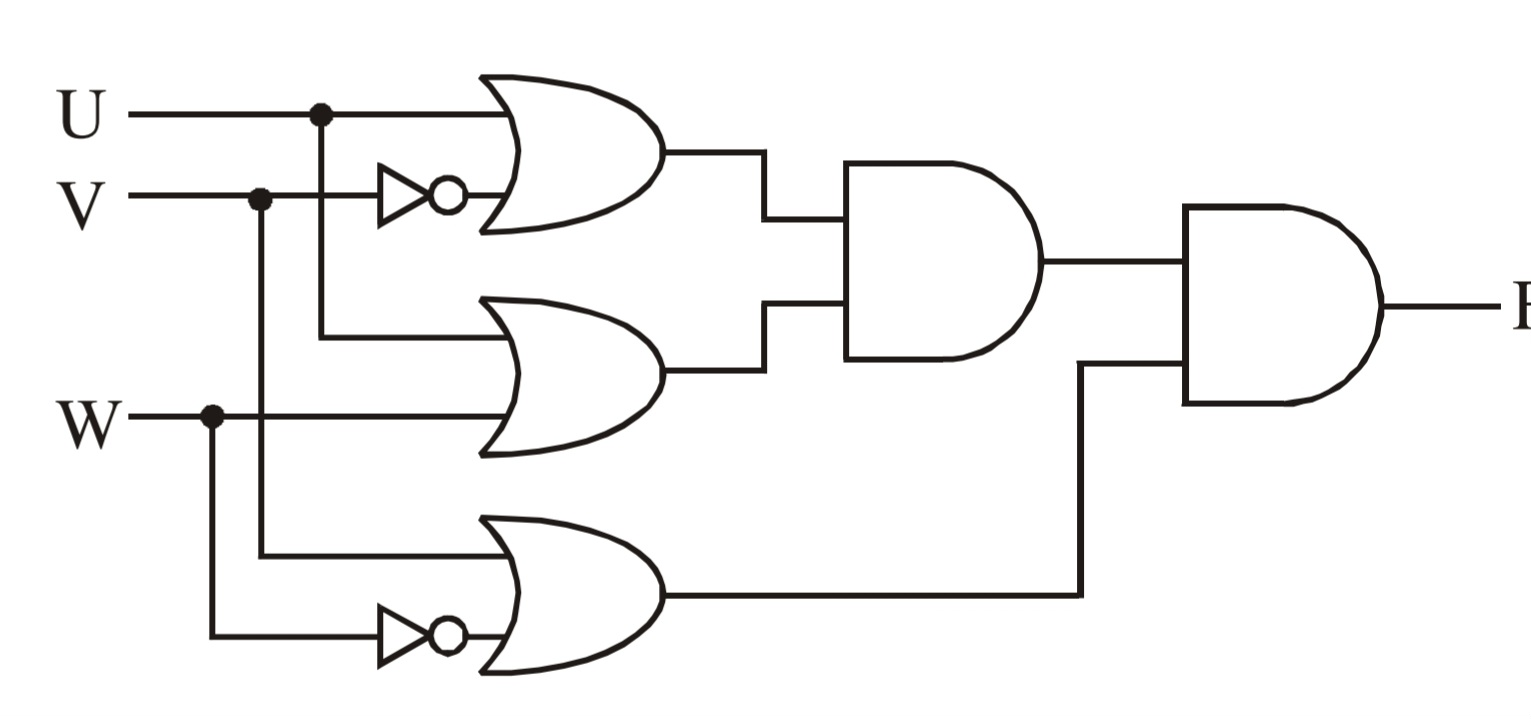
\includegraphics[width=0.5\columnwidth]{figs/cbse-2016.jpg}
\caption{}
\label{fig:2016/c/6/b}
\end{figure}
\item 
Obtain the Boolean Expression for the logic circuit shown below
in \figref{fig:1993/gate/ec/4/8}.
\label{prob:1993/gate/ec/4/8}

\hfill (GATE EC 1993)
\begin{figure}[H]
    \centering
    \resizebox{0.5\columnwidth}{!}{%
	   \begin{circuitikz} \draw
(0,2) node[nand port] (mynand1) {}
(2,3) node[nand port] (mynand2) {}
(0,0) node[nand port] (mynand) {}
(2,-1) node[nand port] (mynand3) {}
(2,1) node[or port] (myor1) {}
(4,1) node[or port,number inputs =3] (myor2) {}
(mynand1.out) -- (myor1.in 1)
(mynand.out) -- (myor1.in 2)
(mynand2.out) -- (myor2.in 1)
(mynand3.out) -- (myor2.in 3)
(myor1.out) -- (myor2.in 2);
\node[left] at (mynand1.in 1) {\(A\)};
\node[left] at (mynand1.in 2) {\(B\)};
\node[left] at (mynand2.in 1) {\(A\)};
\node[left] at (mynand2.in 2) {\(A\)};
\node[left] at (mynand3.in 1) {\(C\)};
\node[left] at (mynand3.in 2) {\(C\)};
\node[left] at (mynand1.in 1)[ocirc] {};
\node[left] at (mynand.in 2) [ocirc] {};
\node[left] at (mynand.in 1) {\(B\)};
\node[left] at (mynand.in 2) {\(C\)};
\node[right] at (mynand1.out) {};
\node[right] at (mynand.out) {};
\node[right] at (mynand2.out) {};
\node[right] at (mynand3.out) {};
\node[right] at (myor2.out) {\(Y\)};
\end{circuitikz}
	}
    \caption{}
\label{fig:1993/gate/ec/4/8}
\end{figure}
%
\item Implement Table
\ref{tab:1993/gate/ec/6/13}
using XNOR logic.
\hfill (GATE EC 1993)
\label{prob:1993/gate/ec/6/13}
\begin{table}[H]
	\centering
	\begin{tabular}{|c|c|c|}
		\hline
		\textbf{A}&\textbf{B}&\textbf{Y}\\
		\hline
		0&0&1\\
		\hline
		0&1&0\\
		\hline
		1&0&0\\
		\hline
		1&1&1\\   
		\hline 
	\end{tabular}
	\caption{}
\label{tab:1993/gate/ec/6/13}
\end{table}
\item 
\label{prob:1999-gate-ec-2-11}
For a binary half-sub-tractor having two inputs A and B, find the correct set of logical expressions for the outputs $D =A \text{ minus } B$ and $X$=borrow.
\hfill (GATE EC 1999)
\item
\label{prob:2016/gate/in/19}
Find $F$ in the Digital Circuit given in the figure below
in \figref{fig:2016/gate/in/19}.
\hfill (GATE IN 2016)
\begin{figure}[H]
	\centering
	\resizebox{0.5\columnwidth}{!}{%
\begin{tikzpicture}
% Logic ports
\node[nand port] (a) at (2,1){};
\node[nand port] (b) at (2,4){};
\node[nand port] (c) at (4,0){};
\node[nand port] (d) at (6,3){};
% Connection
\draw (a.in 2) -| (b.in 2);
\draw (b.out) -| (d.in 1);
\draw (a.out) -|  (c.in 1);
\draw (c.out) -| (d.in 2);
\draw (d.out) -- ++(1,0) node[near end,above]{F};
\draw (b.in 1) -- ++(-1.5,0)node[left](In1){X};
\draw (b.in 2) -- ++(-1.5,0)node[left](In3){Y};
\draw (c.in 2) -- ++(-1.5,0)node[left](In3){Z};
% Jump crossing element
1
\end{tikzpicture}
	}
	\caption{}
\label{fig:2016/gate/in/19}
\end{figure}
\item 
\label{prob:2018-gate-CS-4}		
Let $\oplus$ and $\odot$ denote the Exclusive OR and Exclusive NOR operations, respectively.Which one of the following is NOT CORRECT ?
%\ref{prob:2018-gate-CS-4}

\hfill (GATE CS 2018)
%\begin{samepage}
\begin{enumerate}[label=(\Alph*)]
    \item $\overline{P\oplus Q}$ = $ P \odot Q $
    \item $\overline{P} \oplus Q$ = $ P \odot Q $
    \item $\overline{P} \oplus \overline{Q}$ = $ P \oplus Q $
    \item $(P \oplus \overline{P}) \oplus Q$ = $(P \odot \overline{P}) \odot \overline{Q}$
\end{enumerate}
\item Select the Boolean function(s) equivalent to $x + yz$, where $x,y$, and $z$ are Boolean variables, and + denotes logical OR  operation.\hfill(GATE EC 2022)
	\begin{enumerate}[label=(\Alph*)]
		\item $x + z + {xy}$
		\item ${(x + y)}{(x + z)}$
		\item $x + {xy} + {yz}$
		\item $x + {xz} + {xy}$
	\end{enumerate}
\item 
Consider a Boolean gate $D$ where the output $Y$ is related to the inputs $A$ and $B$ as $Y = A + B$, where + denotes logical OR operation. The Boolean inputs 0 and 1 are also available separately. Using instances of only D gates and inputs 0 and 1, select the correct option(s).\hfill{(GATE EC 2022)}
\begin{enumerate}
\item  NAND logic can be implemented
\item  OR logic cannot be implemented
\item  NOR logic can be implemented
\item  AND logic cannot be implemented.
\end{enumerate}
\item 
\label{prob:2018-gate-ee-14}
Find the logic function implemented by the circuit given below 
in 
\figref{fig:2018-gate-ee-14}

\hfill (GATE EE 2018)
\begin{figure}[H]
\centering
	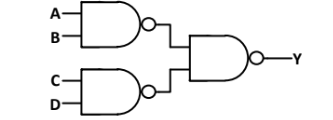
\includegraphics[width=0.5\columnwidth]{figs/2018-gate-ee-14.png}
\caption{}
\label{fig:2018-gate-ee-14}
\end{figure}
%\end{samepage}
\item 
\label{prob:2019-gate-ee-36}
Find the logic function implemented by the circuit given below 
in 
\figref{fig:2019-gate-ee-36}

\hfill (GATE EE 2019)
\begin{figure}[H]
\centering
	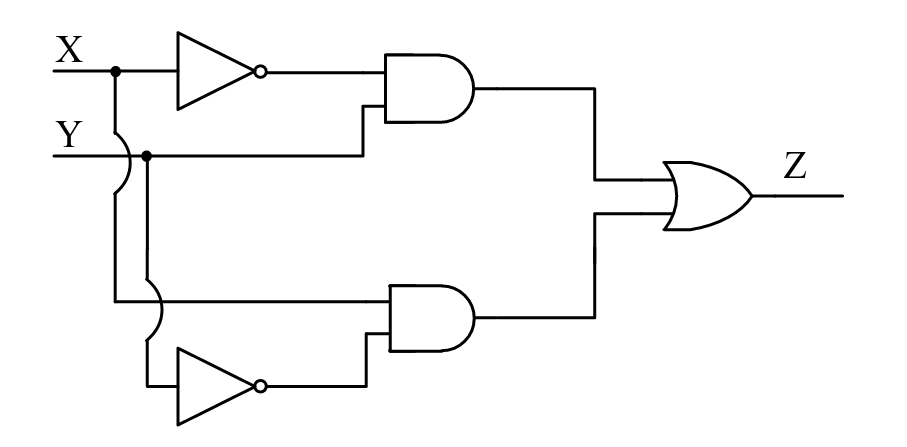
\includegraphics[width=0.75\columnwidth]{figs/2019-gate-ee-36.png}
\caption{}
\label{fig:2019-gate-ee-36}
\end{figure}
 \item Which one of the following options is CORRECT for the given circuit 
			in \figref{fig:xxxx}?
	 \hfill(GATE PHYSICS 2023)
		\begin{figure}[H]
			\centering
			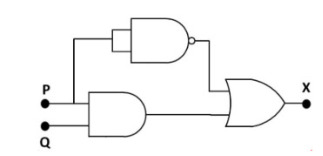
\includegraphics[width=0.5\columnwidth]{figs/Q24.jpg}
			\caption{}
			\label{fig:xxxx}
		\end{figure}

		\begin{enumerate}[label=(\Alph*)]
		\item P = $1$, Q = $1$ ; X = $0$
		\item P = $1$, Q = $0$ ; X = $1$
		\item P = $0$, Q = $1$ ; X = $0$
		\item P = $0$, Q = $0$ ; X = $1$
	\end{enumerate}
%
\item Let $R1$ and $R2$ be two $4$-bit registers that store numbers in $2$’s complement form.
For the operation $R1+R2$, which one of the following values of $R1$ and $R2$ gives an
arithmetic overflow?
\hfill{(GATE CS 2022)}
%
    \begin{enumerate}
        \item $R1 = 1011$ and $R2 = 1110$
        \item $R1 = 1100$ and $R2 = 1010$
        \item $R1 = 0011$ and $R2 = 0100$
        \item $R1 = 1001$ and $R2 = 1111$
    \end{enumerate}
\item The logic block shown 
in
\figref{fig:GATE IN 2021}
	has an output $F$ given by \rule{1cm}{0.5pt}.
\begin{enumerate}
	\item$A+B$
	\item$A\bar{B}$
	\item$A+\bar{B}$
	\item$\bar{B}$
\end{enumerate}
\hfill (GATE IN 2021)
\begin{figure}[H]
\centering
\includegraphics[width=0.5\columnwidth]{figs/gatemage.jpg}
	\caption{}
\label{fig:GATE IN 2021}
\end{figure}
%
\item Consider the following Boolean expression 
\begin{align*} F = (X+Y+Z)(\bar{X}+Y)(\bar{Y}+Z) \end{align*}
%       
Which of the following Boolean expressions is/are equivalent to $\overline{F}$ ?
% 
\begin{enumerate}                                     
\item $(\bar{X}+\bar{Y}+\bar{Z})(X+\bar{Y})(Y+\bar{Z})$
\item $X\bar{Y}+\bar{Z}$
\item $(X+\bar{Z})(\bar{Y}+\bar{Z})$
\item $X\bar{Y}+Y\bar{Z}+\bar{X}\bar{Y}\bar{Z}$ 
\end{enumerate}
\hfill{(GATE CS 2021)}
\item  The following combination of logic gates
in
		      \figref{fig:GATE PH 2021}
	represents the operation
	\begin{enumerate}
       \item OR
       \item NAND
       \item AND
       \item NOR
   \end{enumerate}
%
 \hfill(GATE PH 2021)
	      \begin{figure}[H]
		      \centering
		      \resizebox{0.25\columnwidth}{!}{%
		                   \begin{circuitikz}
              
                  \draw (2,5) node[not port,scale=2] (not) {};
                  \draw (not.in) -- ++(-0.5,0);
                  \draw (not.out) -- ++(0.5,0) ;
                  
                
                
                \draw (7.5,3) node[or port,scale=2] (orgate) {};
                  \draw (orgate.in 1) -- ++(-0.5,0) ;
                  \draw (orgate.in 2) -- ++(-0.5,0);
                  \draw (orgate.out) -- ++(0.5,0) ;
                
                 \draw (2,1) node[not port,scale=2] (notgate) {};
                  \draw (notgate.in) -- ++(-0.5,0) ;
                  \draw (notgate.out) -- ++(0.5,0) ;
                
                \draw (notgate.out) -- ([xshift=0.5cm]notgate.out) |-(orgate.in 2);
                  
                \draw (not.out) -- ([xshift=0.5cm]not.out) |-(orgate.in 1);
                  
            \end{circuitikz}

		      }
	              \caption{}
		      \label{fig:GATE PH 2021}
	      \end{figure}
%
\item In the circuit shown
	in \figref{fig:GATE-EC2019,14},
	what are the values of $F$ for $EN=0$ and $EN=1$,  respectively?
\begin{enumerate}
    \item $0$ and $D$
    \item $Hi-Z$ and $D$
    \item $0$ and $1$
    \item $Hi-Z$ and $\overline{D}$
\end{enumerate}
 \hfill(GATE EC 2019)  
%
\begin{figure}[H]
    \centering
    \resizebox{0.5\columnwidth}{!}{%
    \begin{circuitikz}

\draw (0.5,1) node[nand port] (nand) {};
\draw (nand.in 1) -- ++(-1.7,0) node[left] {};
\draw (nand.in 2) -- ++(-2.2,0) node[left] {EN};
\draw (nand.out) -- ++(0.5,0) node[midway, above] {};
\draw (0.5,-3) node[nor port] (nor) {};
\draw (nor.in 1) node[left] {};
\draw (nor.in 2) --++(-2.2,0) node[left] {D};
\draw (nor.out) -- ++(0.5,0) node[midway, above] {};
\draw (-1.6,-1) node[rotate=270,not port] (not) {};
\draw (not.in) |-(nand.in 2);
\draw  (nor.in 1) -| (not.out);
\draw (2,1) node[pmos] (pmos) {};
\draw (2,-3) node[nmos] (nmos) {};
\draw (nand.out) -- (pmos.gate);
\draw (nor.out) -- (nmos.gate);
\draw(nand.in 1) -- ++(-1.7,0) |- (nor.in 2) -- ++(-1,0);
\draw (pmos.drain) -- (nmos.drain);
\draw (pmos.drain)--++(90:-1)--++(2:1)node[left, yshift=0.2cm]{$F$};
\draw (nmos.source) -- (nmos.source |- 0,-4) node[ground] {};
\draw(2,1.7) node[rground,yscale=-1] {};
\draw(2,2.3) node(right) {$V_{DD}$};

\end{circuitikz}


	}
    \caption{Circuit Diagram}
	\label{fig:GATE-EC2019,14} 
\end{figure}
\item In the circuit shown below in 
	    \figref{fig:GATE-IN2019,34},
	 assume that the comparators are ideal and all components have zero propagation delay. In one period of the input signal $V_{in}=6\sin\brak{\omega t}$, the fraction of the time for which the output OUT is in logic HIGH is 
\begin{enumerate}[itemsep=1ex]
	\item $\frac{1}{12}$
	\item $\frac{1}{2}$
	\item $\frac{2}{3}$
	\item $\frac{5}{6}$
\end{enumerate}
		                 \hfill(GATE IN 2019)
\begin{figure}[H]
\centering
\resizebox{0.75\columnwidth}{!}{%
    \begin{circuitikz}

\draw (0,0) node[op amp] (opamp1) {};
\draw (opamp1.-)  node[left]{};
\draw (opamp1.+) node[left]{};
\draw (opamp1.out) node[right]{} ;
\draw (0,5) node[op amp] (opamp2) {};
\draw (opamp2.-)  node[left]{};
\draw (opamp2.+)  node[left]{};
\draw (opamp2.out) node[right]{};
\draw (3.5,5) node[not port] (notgate1) {};
\draw (notgate1.in) node[left] {};
\draw (notgate1.out) node[right] {};
\draw (3.5,2) node[not port] (notgate2) {};
\draw (notgate2.in) node[left] {};
\draw (notgate2.out) node[right] {};
\draw (6.5,3.5) node[and port] (andgate1) {};
\draw (andgate1.in 1) node[left] {};
\draw (andgate1.in 2)  node[left] {};
\draw (andgate1.out) node[right] {};
\draw (6.5,0.5) node[and port] (andgate2) {};
\draw (andgate2.in 1) node[left] {};
\draw (andgate2.in 2)  node[left] {};
\draw (andgate2.out) node[right] {};
\draw (8,2) node[or port] (orgate) {};
\draw (orgate.in 1) node[left] {};
\draw (orgate.in 2)  node[left] {};
\draw (orgate.out) node[right] {$out$};
\draw (andgate1.out) -| (orgate.in 1);
\draw (andgate2.out) -| (orgate.in 2);
\draw (notgate1.out) -| (andgate1.in 1);
\draw (notgate2.out) -| (andgate1.in 2);
\draw (opamp2.out) -|(notgate1.in);
\draw (opamp1.out) -| (andgate2.in 2);
\draw(opamp2.out)--++(90:0)|-(andgate2.in 1);
\draw(notgate2.in)--++(50:0)|-(opamp1.out);
\draw(opamp1.-)--++(90:0)-|(-3,2)|-(opamp2.-);
\draw(opamp2.+)--++(0,-1) node[rground,rotate=180,yscale=-1]{};
\draw (-1.2,2.8)node(right) {$3V$};
\draw(opamp1.+)--++(0,-1) node[ground,rotate=180,yscale=-1]{};
\draw (-5,5.5) to[sV] (-5,0)node[ground,rotate=180,yscale=-1]{};
\draw (-5,5.5) -- (opamp2.-);
\draw (-6,3)node(right) {$6 \sin{\omega t}$};
\draw (0,5.5) -- (0,6.2)node(right) {};
\draw (0,6.5) node(right) {$HIGH$};
\draw (0,4.5) -- (0,3.8)node(right) {};
\draw(0,3.5) node(right) {LOW};
\draw (0,0.5) -- (0,1.2)node(right) {};
\draw (0,1.5) node(right) {$HIGH$};
\draw (0,-0.5) -- (0,-1.2)node(right) {};
\draw (0,-1.5) node(right) {$LOW$};

\end{circuitikz}


	}
	    \caption{Circuit Daigram}
	    \label{fig:GATE-IN2019,34}
     \end{figure}


\item 
	\figref{fig:GATE-IN2019,22}
	shows the $ith$ full-adder block of a binary adder circuit. $C_i$ is the input carry and $C_{i+1}$is the output carry of the circuit.  If the inputs $A_i, B_i$; are available and stable throughout the carry propagation, find the outputs $S_i$ and $C_{i+1}$.

	               \hfill(GATE IN 2019)
\begin{figure}[H] 
    \centering
    \resizebox{0.75\columnwidth}{!}{%
	\begin{circuitikz}
    \draw (0,0) node[xor port] (xor1) {};
    \draw (xor1.out)  node[right] {};
    \draw (xor1.in 1) -- ++(-0.52,0) node[left] {$B_i$};
    \draw (xor1.in 2) -- ++(-1,0) node[left] {$A_i$};
    
    \draw (5,0) node[xor port] (xor2) {};
    \draw (xor2.out) node[right] {$S_i$};
    \draw (xor2.in 1)  node[left] {};
    \draw (xor2.in 2) |- (2,-2.29) node[below] {$C_i$};
    % First AND gate
    \draw (6,-2) node[and port] (and1) {};
    \draw (and1.out) node[right] {};
    \draw (and1.in 1) node[left] {};
    \draw (and1.in 2)  node[left] {};
    
    % Second AND gate
    \draw (0,-2) node[and port] (and2) {};
    \draw (and2.out)  node[right] {};
    \draw (and2.in 1)  node[left] {};
    \draw (and2.in 2)  node[left] {};
    \draw (9,-3) node[or port] (or) {};
    \draw (or.out) -- ++(0,0) node[right] {$C_{i+1}$};
    \draw (or.in 1) -- ++(-0.5,0) node[left] {};
    \draw (or.in 2) -- ++(-0.5,0) node[left] {};
   \draw (xor1.in 1) -- ++(-0.5,0) |- (and2.in 1);
   \draw (xor1.in 2) -- ++(-1,0) |- (and2.in 2);
    \draw(xor1.out)  --++(1,0)   |- (xor2.in 1);
    \draw(xor2.in 1)--++(-2,0)   |-(and1.in 1);
   % \draw(xor2.in 2)--++(-3,0)   |-(and1.in 2);
    \draw (and1.out)--++(0,-0.7) |-(or.in 1);
     \draw (and2.out)--++(0,-0.7) |-(or.in 2);
     \draw(xor2.in 2) |-(and1.in 2);
    \end{circuitikz}



	}
	\caption{Full Adder}
	\label{fig:GATE-IN2019,22}
\end{figure}
\item  The chip select logic for a certain DRAM chip in a memory system design is shown below
	in
\figref{fig:figure14}.
	Assume that the memory system has 16 address lines denoted by ${A_{15}}$ to ${A_0}$. What is the range of addresses (in hexadecimal) of the memory system that can get enabled by the chip select (CS) signal?
\begin{enumerate}
\item ${C800}$ to ${CFFF}$
\item ${CA00}$ to ${CAFF}$
\item ${CA00}$ to ${C8FF}$
\item ${DA00}$ to ${DFFF}$
\end{enumerate}  
\hfill (GATE CS 2019)
%
\begin{figure}[H]
\begin{center}
\begin{circuitikz}
\draw ((5,5) node[ieeestd and port,number inputs=5,minimum height=5cm, minimum width=5cm, anchor=in 1] (B) {} (B.in 1) node[anchor=east] {$A_{15}$}(B.in 2) node[anchor=east] {$A_{14}$}(B.in 3) node[anchor=east] {$A_{13}$}(B.in 4) node[anchor=east] {$A_{12}$}(B.in 5) node[anchor=east] {$A_{11}$}(B.out) node[anchor=west] {$CS$};
\node at (B.bin 3) [ocirc, left]{} ;
\node at (B.bin 4) [ocirc, left]{};
\end{circuitikz}  
\end{center}
\caption{}
\label{fig:figure14}
\end{figure}
%
\item  A $2\times2$ ROM array is built with the help of diodes as shown in the circuit below
	in \figref{fig:2rom}. Here $W0$ and $W1$ are signals that select the word lines and $B0$ and $B1$ are signals that are output of the sense amps based on the stored data corresponding to the bit lines during the read operation.
%
\begin{figure}[H]
        \centering
	\resizebox{0.75\columnwidth}{!}{%
        \begin{circuitikz} 
\draw (2,0) node[nmos] {} (3,0)
(4,0) node[nmos] {} (5,0)
(4,-0.375) node[ground] {}
(2,-0.375) node[ground] {}
;
\ctikzset{diodes/scale=0.6} 
\draw  (1,3) to[empty diode] (2,2.25)
(3,1.5) to[empty diode ] (4,0.75)
;
\ctikzset{diodes/scale=1} 

\draw [very thick](1.75,3.75) -- (2,4.25) -- (2.25,3.75) -- cycle
(3.75,3.75) -- (4,4.25) -- (4.25,3.75) -- cycle
(0,0) -- (2,0) -- (5,0)
(0,1.5) node[anchor=east] {W1}--  (5,1.5)
(0,0) -- (0,0.625)
(-0.25,1.2) node[anchor=north] {VDD}
(2,4.25) -- (2,4.6) node[anchor=south] {B0}
(4,4.25) -- (4,4.6) node[anchor=south] {B1}
(-0.15,0.55) -- (0,0.625) --(0.15,0.7)
(0,3) node[anchor=east] {W0}  -- (5,3)
(2,0.25) --  (2,3.75)
(4,0.25) -- (4,3.75)
(8.125,1.75) -- (8,1.75) -- (8,3) --(8.125,3)
(9.625,1.75) -- (9.75,1.75) -- (9.75,3) --(9.625,3);
\node (mynode) at (3,4) {\scalebox{0.5}{Sense amps}};
 \filldraw[fill=black, draw=black] (1,3) circle [radius=0.1];
 \filldraw[fill=black, draw=black] (2,2.25) circle [radius=0.1];
 \filldraw[fill=black, draw=black] (3,1.5) circle [radius=0.1];
 \filldraw[fill=black, draw=black] (4,0.75) circle [radius=0.1];
 %matrix code
\node at (8.5,3.5) {$B_{0}$};
\node at (9.25,3.5) {$B_{1}$} ;
\node at (7.4,2.75) {$W_{0}$};
\node at (8.5,2.75) {$D_{00}$};
\node at (9.25,2.75) {$D_{01}$};
\node at (7.4,2) {$W_{1}$};
\node at (8.5,2) {$D_{10}$};
\node at (9.25,2) {$D_{11}$};
\node at (8.7,1) {Bits stored in the ROM Array};


\end{circuitikz}

	}
        \caption{ $2\times 2$ ROM array}
	\label{fig:2rom}
\end{figure}
%
		During the read operation, the selected word line goes high and the other word line is in a high impedance state. As per the implementation shown in the circuit diagram above, what are the bits corresponding to $D_{ij}\brak{\text{where $i=0$ or $1$ and $j=0$ or $1$}}$ stored in the ROM?
	\hfill(GATE EC 2018)
	\begin{multicols}{4}
\begin{enumerate}
    \item \myvec{1 & 0\\0 & 1}
    \item \myvec{0 & 1\\1 & 0}
    \item \myvec{1 & 0\\1 & 0}    
    \item \myvec{1 & 1\\0 & 0}
\end{enumerate}
	\end{multicols}
%
\item $A$ and $B$ are logical inputs and $X$ is the logical output shown in 
\figref{fig:gate_in_2017_30}.
	The output $X$ is related to $A$ and $B$ by 
\begin{enumerate}
\item $X = \overline{A}B + \overline{B}A$
\item $X = AB + \overline{B}A$
\item $X = AB + \overline{B}\overline{A}$
\item $X = \overline{A}\overline{B} + \overline{B}A$
\end{enumerate}
\hfill (GATE IN 2017)
\begin{figure}[H]
\centering
\resizebox{0.75\columnwidth}{!}{%
\begin{circuitikz}
\tikzstyle{every node}=[font=\normalsize]
\draw (7.75,11.5) node[ieeestd not port, anchor=in](port){} (port.out) to[short] (10.5,11.5);
\draw (port.in) to[short] (6.5,11.5);
\draw (7.75,9.5) node[ieeestd not port, anchor=in](port){} (port.out) to[short] (10.25,9.5);
\draw (port.in) to[short] (6.75,9.5);
\draw (11.75,10.75) to[short] (12,10.75);
\draw (11.75,10.25) to[short] (12,10.25);
\draw (12,10.75) node[ieeestd and port, anchor=in 1, scale=0.89](port){} (port.out) to[short] (14,10.5);
\draw (8,7.5) to[short] (8.25,7.5);
\draw (8,7) to[short] (8.25,7);
\draw (8.25,7.5) node[ieeestd and port, anchor=in 1, scale=0.89](port){} (port.out) to[short] (10,7.25);
\draw (14,10.5) to[short] (14,10.5);
\draw (14,10) to[short] (14,10);
\draw (14,10.5) node[ieeestd or port, anchor=in 1, scale=0.89](port){} (port.out) to[short] (15.75,10.25);
\draw[] (6.75,9.5) to[short] (4.25,9.5);
\draw [](5.75,9.5) to[short] (5.75,7);
\draw[] (8,7) to[short] (5.75,7);
\draw[] (8,7.5) to[short] (6.5,7.5);
\draw [](6.5,8) to[short] (6.5,7.5);
\draw[] (11.75,10.75) to[short] (10.5,10.75);
\draw[] (11.75,10.25) to[short] (10.5,10.25);
\draw [](10.5,10.25) to[short] (10.5,9.5);
\draw[] (10.5,9.5) to[short] (10.25,9.5);
\draw [](14,10) to[short] (14,7.5);
\draw [](10,7.25) to[short] (14,7.25);
\draw [](14,7.25) to[short] (14,7.75);
\draw [](10.5,11.5) to[short] (10.5,10.75);
\draw[] (6.5,11.5) to[short] (4.25,11.5);
\draw [](6.5,8) to[short] (6.5,9.25);
\draw [](6.5,11.5) to[short] (6.5,9.75);
\draw [](6.5,10) to[short] (6.5,9.25);
\draw [](4.25,9.5) to[short, -o] (3.75,9.5);
\draw [](4.25,11.5) to[short, -o] (3.75,11.5);
\node [font=\normalsize] at (3.5,11.5) {A};
\draw [](15.75,10.25) to[short, -o] (16.25,10.25);
\node [font=\normalsize] at (3.5,9.5) {B};
\node [font=\normalsize] at (16.5,10.25) {X};
\draw (5.75,9.5) to[short, -*] (5.75,9.5);
\draw (6.5,11.5) to[short, -*] (6.5,11.5);
\end{circuitikz}

	}
\caption{}
\label{fig:gate_in_2017_30}
\end{figure}
% 
\item 
Which one the following is not a valid identity?
\begin{enumerate}
 \item $ (x\oplus y)\oplus z = x\oplus (y\oplus z)$
 \item $ (x + y)\oplus z = x\oplus (y + z)$
 \item $ x\oplus y = x + y, xy = 0$
 \item $ x\oplus y = (xy + x'y')'$
\end{enumerate}
\hfill{(GATE CS 2019)}
        \item Let $p$ and $q$ be two propositions. Consider the following two formulae in propositional logic.
			\begin{align*}
				 S_1 : ( \rightharpoondown p \vee (p \wedge q))\rightarrow q \\
				 S_2 : q\rightarrow(\rightharpoondown p \vee (p \wedge q))
			\end{align*}
        Which one of the following choices is correct?
		\begin{enumerate}
			\item Both $S_1$ and $S_2$ are tautologies.
			\item $S_1$ is a tautology but $S_2$ is not a tautology.
			\item $S_1$ is not a tautology but $S_2$ is a tautology.
			\item Neither $S_1$ nor $S_2$ is a tautology.
		\end{enumerate}
		                                          \hfill(GATE CS 2021)
\item The functionality implemented by the circuit below 
in
\figref{fig:gate_ec_2016_43}
	is 
\begin{enumerate}
\item 2-to-1 multiplexer
\item 4-to-1 multiplexer
\item 7-to-1 multiplexer
\item 6-to-1 multiplexer
\end{enumerate}
\hfill (GATE 2016 EC)
%
\begin{figure}[H]
\centering
\resizebox{0.5\columnwidth}{!}{%

\begin{circuitikz}[scale=1.1]
\tikzstyle{every node}=[font=\large]
\draw  (5,10.75) rectangle (7.75,7);
\draw [](4.75,16) to[short] (11.75,16);
\draw [](4.75,14.75) to[short] (11.75,14.75);
\draw [](4.75,13.25) to[short] (11.75,13.25);
\draw [](4.75,17.5) to[short] (11.75,17.5);
\draw (11.5,17.5) node[ieeestd buffer port, anchor=in](port){} (port.out) to[short] (13.25,17.5);
\draw (port.in) to[short] (11.25,17.5);
\draw (11.5,16) node[ieeestd buffer port, anchor=in](port){} (port.out) to[short] (13.5,16);
\draw (port.in) to[short] (11,16);
\draw (11.5,14.75) node[ieeestd buffer port, anchor=in](port){} (port.out) to[short] (13,14.75);
\draw (port.in) to[short] (11.5,14.75);
\draw (11.5,13.25) node[ieeestd buffer port, anchor=in](port){} (port.out) to[short] (13.25,13.25);
\draw (port.in) to[short] (11.25,13.25);
\draw [](12.25,17.25) to[short] (12.25,16.75);
\draw[] (12.25,16.75) to[short] (9.25,16.75);
\draw [](9.25,16.75) to[short] (9.25,10.25);
\draw[] (9.25,10.25) to[short] (7.75,10.25);
\draw [](12.25,15.75) to[short] (12.25,15.5);
\draw[] (12.25,15.5) to[short] (10,15.5);
\draw [](10,15.5) to[short] (10,9.75);
\draw[] (10,9.75) to[short] (7.75,9.75);
\draw [](12.25,14.5) to[short] (12.25,14);
\draw[] (12.25,14) to[short] (10.75,14);
\draw [](10.75,14) to[short] (10.75,9.25);
\draw [](10.75,9.25) to[short] (10.75,8.75);
\draw[] (10.75,8.75) to[short] (7.75,8.75);
\draw [](12.25,13) to[short] (12.25,7.75);
\draw[] (12.25,7.75) to[short] (7.75,7.75);
\draw [](4,10) to[short] (5,10);
\draw [](4,8) to[short] (5,8);
\draw [](13.25,17.5) to[short] (13.75,17.5);
\draw [](13.75,17.5) to[short] (13.75,13.25);
\draw [](13.25,13.25) to[short] (13.75,13.25);
\draw [](13,14.75) to[short] (13.75,14.75);
\draw [](13.5,16) to[short] (13.75,16);
\draw [](13.75,15.5) to[short] (15.25,15.5);
\node [font=\LARGE] at (4.75,18) {P};
\node [font=\LARGE] at (4.75,16.75) {Q};
\node [font=\LARGE] at (4.75,15.25) {R};
\node [font=\LARGE] at (4.75,13.75) {S};
\node [font=\LARGE] at (3.75,10.5) {$C_1$};
\node [font=\LARGE] at (3.5,8.5) {$C_2$};
\node [font=\LARGE] at (15.25,15.75) {Y};
\node [font=\LARGE] at (8.75,10.75) {$O_0$};
\node [font=\LARGE] at (9,9.25) {$O_1$};
\node [font=\LARGE] at (9,8.25) {$O_2$};
\node [font=\LARGE] at (8.75,6.75) {$O_3$};
\draw [](6.25,7) to[short] (6.25,5.25);
\node [font=\large] at (4.5,6) {Enable=1};
\end{circuitikz}


	}
\caption{Multiplexer}
\label{fig:gate_ec_2016_43}
\end{figure}
%
\item A 3-input majority gate is defined by the logic function 
	$$M(a, b, c) = ab + bc + ca.$$ Which one of the following gates is represented by the function $$M\overline{(M(a, b, c)}, M(a, b, \overline{c}), c)?$$
\begin{enumerate}
    \item 3-input NAND gate 
    \item 3-input XOR gate 
    \item 3-input NOR gate 
    \item 3-input XNOR gate 
\end{enumerate}
    \hfill(GATE EC 2015)
%
\item A $2$-bit flash Analog to Digital Converter (ADC) is given in \figref{EE2016_37_fig1}. The input is $0 \leq V_{IN} \leq 3$ Volts. The expression of the LSB of the output $B_0$ as a boolean function of $X_2,X_1,$ and $X_0$ is 
\begin{enumerate}
\item $X_0 \left[ \overline {X_2 \oplus X_1} \right]$
\item $\overline {X_0} \left[ \overline {X_2 \oplus X_1} \right]$
\item $X_0 \left[ X_2 \oplus X_1 \right]$
\item $\overline{X_0} \left[ X_2 \oplus X_1 \right]$
\end{enumerate}
\hfill(GATE EE 2016)
\begin{figure}[H]
\centering
\resizebox{0.5\columnwidth}{!}{%
\begin{circuitikz}[american voltages, american resistors]
    % Resistor network and voltage source
    \draw
    (0,9.5) -- (0,10) node[above] {$3V$}
    to[R, l=100$\Omega$] (0,7) % Resistor 100 Ohm
    to[R, l=200$\Omega$] (0,4) % Resistor 200 Ohm
    to[R, l=200$\Omega$] (0,1) % Resistor 200 Ohm
    to[R, l=100$\Omega$] (0,-2); % Resistor 100 Ohm
    
    % Nodes for the tap points
    \node at (0,7) [circle,fill,inner sep=2pt]{};
    \node at (0,4) [circle,fill,inner sep=2pt]{};
    \node at (0,1) [circle,fill,inner sep=2pt]{};

    % Op-amps with feedback loop as in the provided design
    % Op-amp 2
    \draw (6,6.5) node[op amp, noinv input up] (opamp2) {}
    (opamp2.+) to[short] ++(-1.25,0) to[short] ++(0,-4)
    (opamp2.-) to[short] ++(-3.25,0) to[short] ++(0,1) to[short] ++(-1.5,0);
    % Power supply connections
    \draw (opamp2.up) -- ++(0,0.4);
    \draw (opamp2.down) -- ++(0,-0.4)
    (opamp2.out) to[short] ++(0,0) node[above] {$X_2$} -- ($(opamp2.out)+(0.5,0)$);
    
    % Op-amp 1
    \draw (6,3.5) node[op amp, noinv input up] (opamp1) {}
    (opamp1.+) to[short] ++(-1.25,0) to[short] ++(0,-4)
    (opamp1.-) to[short] ++(-3.25,0) to[short] ++(0,1) to[short] ++(-1.5,0);
    % Power supply connections
    \draw (opamp1.up) -- ++(0,0.4);
    \draw (opamp1.down) -- ++(0,-0.4)
    (opamp1.out) to[short] ++(0,0) node[above] {$X_1$} -- ($(opamp1.out)+(0.5,0)$);
    
    % Op-amp 0
    \draw (6,0.5) node[op amp, noinv input up] (opamp0) {}
    (opamp0.+) to[short] ++(-1.25,0) to[short] ++(0,-2.5) node[ above right] {$V_{IN}$}
    (opamp0.-) to[short] ++(-3.25,0) to[short] ++(0,1) to[short] ++(-1.5,0);
    % Power supply connections
    \draw (opamp0.up) -- ++(0,0.4);
    \draw (opamp0.down) -- ++(0,-0.4)
    (opamp0.out) to[short] ++(0,0) node[above] {$X_0$} -- ($(opamp0.out)+(0.5,0)$);

    % Nodes for the tap points
    \node at (3.55,7) [circle,fill,inner sep=2pt]{};
    \node at (3.55,4) [circle,fill,inner sep=2pt]{};
    \node at (3.55,1) [circle,fill,inner sep=2pt]{};

    % Digital circuit block
    \draw[thick] ($(opamp2.out)+(0.5,0.5)$) rectangle ($(opamp0.out)+(2,-0.5)$);
    \node at (8.425,3.5) {Digital};
    \node at (8.425,3.2) {Circuit};

    % Outputs from the digital circuit
    \draw ($(opamp2.out)+(2,-2.5)$) -- ++(0.5,0) node[right] {$B_1$};
    \draw ($(opamp0.out)+(2,2.5)$) -- ++(0.5,0) node[right] {$B_0$};

\end{circuitikz}

	}
\caption{}
\label{EE2016_37_fig1}
\end{figure}
\item 
In
\figref{fig:GATE-EE 2018,47},
the number of distinct values of $X_3X_2X_1X_0$ (out of the $16$ possible values) that give $Y=1$ is \rule{1cm}{0.5pt}.
\hfill(GATE EC 2018)
\begin{figure}[H]
\centering
\resizebox{0.75\columnwidth}{!}{%
\begin{circuitikz}
    %Input nodes
    \draw(0,3) node[left] (p) {$X_0$};
    \draw(0,0.7) node[left] (q) {$X_1$};
    \draw(0,0.3) node[left] (r) {$X_2$};
    \draw(0,-1) node[left] (s) {$X_3$};

    %co-ordinates
    \draw(0.5,2) coordinate(a);
    \draw(0.5,-2) coordinate(b);
    \draw(2.6,1.6) coordinate(c);
    \draw(5.1,3) coordinate(d);

    %NOT Gate
    \draw(2,3) node[not port,scale=0.75] (notp) {};
    \draw(2,-1) node[not port,scale=0.75] (nots) {};

    %XOR Gate
    \draw(2.5,0.5) node[xor port,scale=0.75](xor){};
    
    %AND Gate
    \draw(5,1.8) node[and port,scale=0.75](and){};
    
    %OR node
    \draw(8,-0.8) node[or port,scale=0.75](or){};
    
    %Output node
    \draw(or.out) --++(1,0) node[near end,above](y){$Y$};

    %Connect nodes
    \draw(p) -- (notp.in);
    \draw(q) -|(xor.in 1);
    \draw(r) -|(xor.in 2);
    \draw(s) -- (nots.in);
    \draw(a) -| (and.in 1);
    \draw(a) to [short,-*] (0.5,3);
    \draw(nots.out) -| (xor.out);
    \draw(c) -| (and.in 2);
    \draw (c) to [short,-*] (2.6,0.5);
    \draw(b) to [short,-*](0.5,-1);
    \draw(b) -| (or.in 2);
    \draw(d) -- (notp.out);
    \draw(d) to [short,-*] (and.out);
    \draw(and.out) -| (or.in 1);
    
\end{circuitikz}

	}
	\caption{}
\label{fig:GATE-EE 2018,47}
\end{figure}
\item In the circuit shown in 
\figref{fig:GATE-EC 2014,15},
 if $C = 0$, the expression for $Y$ is
\begin{enumerate}
    \item $Y= A\overline{B}+ \overline{A}B $ 
    \item $Y=A+B$
    \item $Y=\overline{A}+\overline{B}$
    \item $Y=AB$
\end{enumerate}
\hfill (GATE EC 2014)
\begin{figure}[H]
\centering
\resizebox{0.75\columnwidth}{!}{%
\begin{circuitikz}

 % Input nodes
 \draw (0,0) node[left] (C){$C$};

  %co-ordinates
\draw(1,-2.71) coordinate(a);
\draw(1,0) coordinate(b);
\draw(6.65,0) coordinate(q);
\draw(6.65,-2.3) coordinate(r);

   
    % NOT gates
\draw (5,0) node[not port,scale=0.75] (notx){};
    

    % NOR gates
\draw (3,-1) node[nor port,scale=0.75] (norx){};

   % OR gate
   
\draw (5,-2.5) node[or port,scale=0.75] (orx){};
\draw (6.5,-4) node[or port,scale=0.75] (ory){};


  % AND gates
\draw (4.5,-4.19) node[and port,scale=0.75] (andx){};

     % NAND gates
\draw (8.5,-2.5) node[nand port,scale=0.80] (nandx){};

 % Connect nodes
\draw (C) -- (notx.in);
\draw (norx.out) |- (orx.in 1);
\draw (orx.out) -| (ory.in 1);
\draw (ory.out) |- (nandx.in 2);
\draw (notx.out) --(q);
\draw (q) --(r);
\draw (r) --(nandx.in 1);
 
\draw (andx.out) -- (ory.in 2);
\draw (a) -- (orx.in 2);
\draw (a) -- (b);
 % inputs and output ports
\draw (nandx.out) -- ++(0.5,0) node[right](d){$Y$};
\draw (norx.in 1) -- ++(-0.2,0) node[left](e){$A$};
\draw (norx.in 2) -- ++(-0.2,0) node[left](f){$B$};
\draw (andx.in 1) -- ++(-0.2,0) node[left](g){$A$};
\draw (andx.in 2) -- ++(-0.2,0) node[left](g){$B$}; 
 
\end{circuitikz}

	}
	\caption{}
\label{fig:GATE-EC 2014,15}
\end{figure}
\item In the logic circuit shown in  
\figref{fig:GATE-EE 2018,14},
	$Y$ is given by
\hfill(GATE EE 2018)
\begin{enumerate}
    \item $Y = ABCD$
    \item $Y = ( A + B)(C + D) $
    \item $Y = A +B +C+ D$
    \item $Y = AB+CD $
\end{enumerate}
\begin{figure}[H]
\centering
\resizebox{0.5\columnwidth}{!}{%
\begin{circuitikz}
        %Input nodes
\draw(0,3.7) node[left](a) {$A$};
\draw(0,3.3) node[left](b) {$B$};
\draw(0,1.7) node[left](c) {$C$};
\draw(0,1.3) node[left](d) {$D$};
%nand
\draw(2.5,3.5) node[nand  port,scale=0.75](nand 1){};
\draw(2.7,1.5) node[nand  port,scale=0.75](nand 2){};
\draw(4,2.5)   node[nand  port,scale=0.75](nand 3){};
%output
\draw(nand 3.out) -- ++(1,0) node[near end,above](y){$Y$};
%Connect nodes
\draw(a) -| (nand 1.in 1);
\draw(b) -| (nand 1.in 2);
\draw(c) -| (nand 2.in 1);
\draw(d) -| (nand 2.in 2);
\draw(nand 3.in 1) -| (nand 1.out);
\draw(nand 3.in 2) -| (nand 2.out);
\end{circuitikz}

	}
	\caption{}
\label{fig:GATE-EE 2018,14}
\end{figure}
%
\item The logic function $f\brak{X,Y}$ realised by the given circuit in
\figref{fig:GATE-EC 2018,8}
is
\begin{enumerate}
    \item NOR
    \item AND
    \item NAND
    \item XOR
\end{enumerate}
\hfill (GATE EC 2018)
\begin{figure}[H]
\centering
\resizebox{0.75\columnwidth}{!}{%
\begin{circuitikz}
    
    \draw (0,0) node[left] (x1) {$X$};
    \draw (2,0) node[not port,scale=0.75] (not1) {};
    \draw (x1) --(not1.in);
    \draw (5,0) node[pmos](pmos1){};
    \draw (not1.out) -- (pmos1.G);
    \draw (pmos1.S) -- (6,0.75)-- (6,1.5)node[vcc] {$V_{\text{DD}}$};
    \draw (7,0)node[pmos ,xscale=-1](pmos3){};
    \draw (6,0.75) -- (pmos3.S);
    \draw (10,0) node[right] (x2) {$X$};
    \draw (pmos3.G) -- (x2);
    \draw (5,-1.5) node[pmos](pmos2){};
    \draw (pmos1.D) -- (pmos2.S);
    \draw (0,-1.5) node[left](y1) {$Y$};
    \draw (y1) -- (pmos2.G);
    \draw (7,-1.5) node[pmos ,xscale=-1](pmos4){};
    \draw (pmos3.D) -- (pmos4.S);
    \draw (8.5,-1.5)node[not port,scale=0.75,rotate=180] (not3){};
    \draw (pmos4.G) -- (not3.out);
    \draw (10,-1.5) node[right] (y2){$Y$};
    \draw (not3.in) -- (y2);
    \draw (pmos2.D) -- (pmos4.D);
    \draw (6,-2.25) -- (6,-3.75);

    \draw (5,-4.5)node[nmos](nmos1){};
    \draw (5,-6)node[nmos](nmos2){};
    \draw (nmos1.S) -- (nmos2.D);
    \draw (3,-6) node[not port,scale=0.75] (not2) {};
    \draw (3,0) -- (3,-4.5);
    \draw (3,-4.5) -- (nmos1.G);
    \draw (2,-1.5) -- (2,-6);
    \draw (2,-6) -- (not2.in);
    \draw (not2.out) -- (nmos2.G);

    \draw (7,-4.5)node[nmos ,xscale=-1](nmos3){};
    \draw (nmos3.G) -- (9.5,-4.5);
    \draw (9.5,-4.5) -- (9.5,0);
    \draw (7,-6)node[nmos ,xscale=-1](nmos4){};
    \draw (nmos4.G) -- (9,-6);
    \draw (9,-6)--(not3.in);
    \draw (nmos2.S) -- (nmos4.S);
    \draw (6,-6.75)-- (6,-7)node[ground]{};
    \draw (nmos1.D) --(nmos3.D);
    
    \draw (6,-3)--(7,-3) node[right] (output){$f\brak{X,Y}$};    
\end{circuitikz}

	}
	\caption{}
\label{fig:GATE-EC 2018,8}
\end{figure}
%
\item $P, Q$ and $R$ are the decimal integers corresponding to the  $4$-bit binary number  $1100$ considered in single magnitude, $1$'s complement and $2$'s complement representations, respectively. The $6$-bit $2$'s complement representation of $\brak{P + Q + R}$ is
\begin{enumerate}
  \item $110101$
  \item $110010$
  \item $111101$
  \item $111001$
\end{enumerate}
   \hfill(GATE EC 2020)
%
\item In the circuit shown below
	in
\figref{prob:gate  ec2023,23 },
	 $P$ and $Q$ are the inputs. The logical function realized by the circuit 
is \rule{1cm}{0.1pt}.
\hfill(GATE EC 2023)
   \begin{enumerate}
    \item Y=PQ
    \item Y=P+Q    
    \item Y= $\overline{PQ}$
    \item Y= $\overline{P+Q}$
\end{enumerate}
\begin{figure}[H]
\centering
\resizebox{0.5\columnwidth}{!}{%
\begin{circuitikz}
\draw (0,0) --(8,0)--(8,8)--(0,8)-- cycle;
 % Draw the input lines
 \draw (0,1.6) -- (-2.0,1.6) node [left] {$P$};
\draw (0,1.6)  (0.6,1.6) node [right] {$I_1$};
\draw (0,6.4) -- (-2.0,6.4) to[ground](-2,5);
\draw (-3,5)--(-1,5);
\draw (-2.7,4.8)--(-1.3,4.8);
\draw (-2.4,4.6)--(-1.6,4.6);
\draw (0,6.4) (0.6,6.4) node [right] {$I_0$};
\draw (3.7,0)  (3.7,0.5) node [right] {$Sel$};
\draw(4,0)--(4,-2)--cycle;(-4,-2)--cycle;
\draw(-2,-2)--(4,-2)--cycle;
\draw (-0.8,-2)-- (-2,-2) node [left] {$Q$};
    
 % Draw the output line
\draw (8,4.0) -- (9,4.0) node [right] {Y};
% Draw the multiplexer symbol
\draw (3.7,4.0)  node{$2$};
\draw (4.0,4.0)  node{x};
\draw (4.3,4.0)  node{$1$};
\draw (4.0,3.4)  node{MUX};
\end{circuitikz}
	}
	\caption{}
\label{prob:gate  ec2023,23 }
\end{figure}
\item
        In \figref{fig:gate23_ph24}, which of the following is correct?
\hfill(GATE PH 2023)
\begin{enumerate}
    \item P = 1, Q = 1; X = 0
    \item P = 1, Q = 0; X = 0
    \item P = 0, Q = 1; X = 0
    \item P = 0, Q = 0; X = 1
\end{enumerate}
%
\begin{figure}[H]
        \centering
        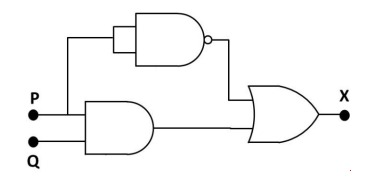
\includegraphics[width=0.5\columnwidth]{ide/kmap/figs/gate23_ph24.jpg}
        \caption{}
        \label{fig:gate23_ph24}
    \end{figure}  
\item 
	\label{prob:2022/gate/in/21}
	The logic block shown in
                \figref{fig:circuit}
	has an output F given by \rule{10mm}{0.4pt}.	
        \begin{enumerate}
                \item $ A + B $
                \item $ A \bar{B} $
                \item $ A + \bar{B} $
                \item $ \bar{B} $
        \end{enumerate}
		\hfill(GATE IN 2022)
	\begin{figure}[H]
                \centering
		\resizebox{0.5\columnwidth}{!}{%
                \begin{circuitikz}
                        \draw
                        (0,0) 
                        node[label=left:$B$] {}
                        -- (7,0)
                        (3,0.75) 
                        node[not port, anchor=out, scale=0.75] (not1) {}
                        (1,0) to[short, *-] (1,0.75) -- (not1.in)
                        (0,-2) node[label=left:$A$] {} -- (7,-2)
                        (3,-1.25) node[not port, anchor=out, scale=0.75] (not2) {}
                        (1,-2) to[short, *-] (1,-1.25) -- (not2.in)
                        (3,0.75) -- (7,0.75)
                        (3,-1.25) -- (7,-1.25)
                        (3.5,-1.25) to[short, *-] (3.5,-3.5)
                        (3.5,-3.5) node[nor port, rotate=270, anchor=in 2] (gate1) {}
                        (gate1.in 1)
                        to[short, -*] ++(0,4.25)
                        (5.5,-2) to[short, *-] (5.5,-3.5)
                        (5.5,-3.5) node[nor port, rotate=270, anchor=in 2] (gate2) {}
                        (gate2.in 1)
                        to[short, -*] ++(0,4.25)
                        (4.75,-6.5) node[nor port, rotate=270] (gate3) {}
                        (gate3.in 2) |- (gate1.out)
                        (gate3.in 1) |- (gate2.out)
                        (gate3.out) -- (4.75,-7) node[label=below:$F$] {};
                \end{circuitikz}
		}
                \caption{}
                \label{fig:circuit}
	\end{figure}
\item In the circuit shown below in 
	\figref{fig},
	 X and Y are digital inputs, and Z is a digital output. The equivalent 
		circuit is a  
		\hfill(GATE EE 2019)
		\label{prob:2019 EE 36}
    \begin{enumerate}
        \item NAND gate
        \item NOR gate
        \item XOR gate
        \item XNOR gate
    \end{enumerate}
\begin{figure}[H]
    \centering
    \resizebox{0.75\columnwidth}{!}{%
    \begin{circuitikz}[scale=1]
    % 1st not
        \draw (0,0) node[not port,scale=0.8 ] (not) {};
        \draw (3,-0.28) node[and port] (and) {};
        
        \draw (not.in 1) -- ++(-1,0) node[left] {$X$};
        \draw (not.out) -- ++(0,0) coordinate (and.in 1);
        \draw (not.in 1) -- ++(0,-1.7) node[below] {$ $};
    % 1st And
        \draw (and.in 1) -- ++(-1.2,0) node[left] {$ $};
        \draw (and.in 2) -- ++(-3.3,0) node[left] {$Y$};
        \draw (and.out) -- ++(0,0) node[right] {$ $};

        \draw (and.in 2) -- ++(-3,0) coordinate (point);
        \draw (point) -- ++(0,-1.7) -- ++(1,0) node[below] {$ $};
        \draw (and.out) -- ++(0,-0.47) node[below] {$ $};
    %2nd not
        \draw (0,-2.28) node[not port ,scale=0.8] (not) {};
        \draw (not.in 1) -- ++(-0.8,0) node[left] {$ $};
        \draw (not.out) -- ++(0,0) coordinate (and.in 2);
   %2nd ANd
        \draw (3,-2) node[and port] (and) {};
        \draw (and.in 1) -- ++(-2.2,0) node[left] {$ $} ;
        \draw (and.in 2) -- ++(-1.2,0) node[left] {$ $} ;
        \draw (and.out) -- ++(0,0) node[right] {$ $};
          \draw (and.out) -- ++(0,0.7) node[above] {$ $};
    %or
        \draw (6,-1) node[or port] (or) {};
        \draw (or.in 1) -- ++(-1.48,0) node[left] {$ $} ;
        \draw (or.in 2) -- ++(-1.48,0) node[left] {$ $} ;
        \draw (or.out) -- ++(1,0) node[right] {$Z$};
     \end{circuitikz}
	}
	\caption{ }
	\label{fig}
\end{figure}
\item The minimum number of two-input NAND gates required to implement the Boolean expression 
\begin{align*}
Y=\sbrak{A\bar{B}\brak{C+BD}+\bar{A}\bar{B}}C
\end{align*}
is \rule{1cm}{0.1pt}.
\hfill(GATE-PH-2022)
\item The Boolean expression for the shaded 
regions as shown in 
\figref{fig:figure12}
is $\underline{\hspace{2cm}}$.
\hfill\brak{GATE \enspace IN2020-11}

\begin{figure}[H]
	\centering
	\resizebox{0.75\columnwidth}{!}{%
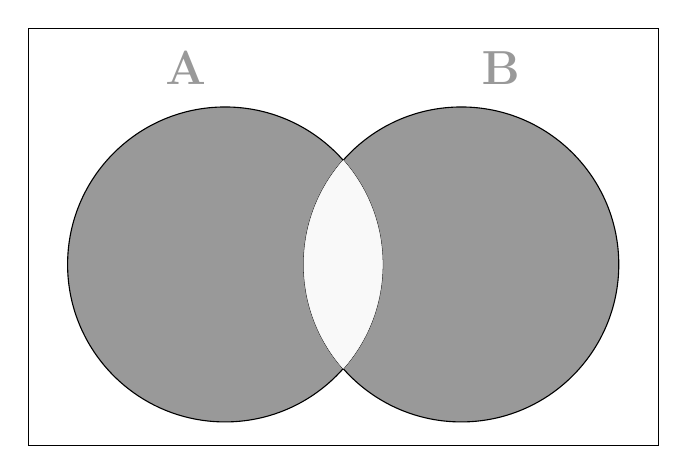
\begin{tikzpicture}
\begin{scope}[fill opacity=.4]
\draw (-4, 4) rectangle (4, -1.3);
\draw[fill=black, draw=black] 
(-1.5, 1) circle (2);
\draw[fill=black, draw=black] 
(1.5, 1) circle (2);
\node at (-2, 3.5) {\LARGE\textbf{A}};
\node at (2, 3.5) {\LARGE\textbf{B}};
\begin{scope}
\clip (-1.5, 1) circle (2);
\clip (1.5, 1) circle (2);
\draw[fill=white, draw=black] 
(-5, 4.5) rectangle (5, -2);
\draw[fill=white, draw=black] 
(-5, 4.5) rectangle (5, -2);
\draw[fill=white, draw=black] 
(-5, 4.5) rectangle (5, -2);
\draw[fill=white, draw=black] 
(-5, 4.5) rectangle (5, -2);
\draw[fill=white, draw=black] 
(-5, 4.5) rectangle (5, -2);
\draw[fill=white, draw=black] 
(-5, 4.5) rectangle (5, -2);
\draw[fill=white, draw=black] 
(-5, 4.5) rectangle (5, -2);
\end{scope}
\end{scope}
\end{tikzpicture}

	}
\caption{Venn Diagram}
\label{fig:figure12}
\end{figure}


\begin{enumerate}
\item $(A + B)\bullet(\overline{A} + \overline{B})$
\item $(A + \overline{B})\bullet(\overline{A} + B)$
\item $(\overline{A} +  B)\bullet
(\overline{A} + \overline{B})$
\item $(\overline{A} + \overline{B})\bullet
(A + \overline{B})$
\end{enumerate}
\item The Boolean operation performed by the following  circuit 
in
\figref{fig:figure13}
	at the output $O$ is \rule{1cm}{0.1pt}.
%
\begin{enumerate}

            \item  $O=S_1\oplus S_0$ 
            
            \item  $O=S_1\overline{\rm S_0}$
            
            \item  $O=S_1 + S_0$
            
            \item $O=S_0\overline{\rm S _1}$
 \end{enumerate}
    \hfill (GATE IN 2020)
%
\begin{figure}[H]
	\centering
	\resizebox{0.75\columnwidth}{!}{%
    \begin{circuitikz}[circuit logic IEC]
        
        \node[and gate, inputs={nnnn}, and gate IEC symbol={}, text height=6cm, text width=3cm] (A) at  (0,0){}; 
        \draw (-2.55,0.62) -- ++(-3.2,0);
        \draw (-2.55,-0.62) -- ++(-3.2,0); 
        \draw (-2.55,-1.85) -- ++(-5.5,0); 
        \draw (-5.7,-0.65) -- ++(0,2.5); 
        \draw (-8,-1.9) -- ++(0,3.72); 
        \node at (0.6,2.5) [anchor=north east] {4:1};
        \node at (0.8,2) [anchor=north east] {Mux};
        \node[anchor=east] at ([xshift=0.6cm]A.input 1) {$I_0$};
        \node[anchor=east] at ([xshift=0.6cm]A.input 2) {$I_1$};
        \node[anchor=east] at ([xshift=0.6cm]A.input 3) {$I_2$};
        \node[anchor=east] at ([xshift=0.6cm]A.input 4) {$I_3$};
       \draw ([xshift=-0.6cm]A.output) node[right] {$O$};

        \draw (A.output) -- ++(0.2,0); 
        \foreach \i in {1,...,4}
            \draw (A.input \i) -- ++(-1,0);
        \draw (A.output) -- ++(1,0);
        \node[not port] (not_gate) at (-4.5,1.85) {};
        \draw (not_gate.out) -- ++(1.2,0);
        \draw (not_gate.in) -- ++(-1,0);
        \node[not port] (not_gate) at (-6.9,1.85) {};
        \draw (not_gate.in) -- ++(-1.9,0);
        \draw (-9.49,-1.67) -- ++(0,3.5); 
        \draw (-9.49,-1.67) node[ground] {};
        \path (A.south) -- ++(0,-0.5) coordinate (bottom_center);
    
        \draw (A.south) ++(-0.5,0) -- ++(0,-0.5) node[below] {$s_1$};
        \draw (A.south) ++(0.5,0) -- ++(0,-0.5) node[below] {$s_0$};
      
        \node[below] at ($(A.south) + (-0.7,-0.9)$) {MSB};
       
        \node[below] at ($(A.south) + (0.7,-0.9)$) {LSB};
    \end{circuitikz}

	}
\caption{}
\label{fig:figure13}
\end{figure}

\end{enumerate}


